

\section{Discussion}

\subsection{Explaining Traversal Variations in Chemistry}

Increasing DSi concentration with decreasing elevation suggests the springs are sampling increasingly longer flow paths. This is because longer flow paths allow for more water-rock interaction, which scavenges more Si from the silicate rocks. While most traverses show such a trend, this does not happen in Traverse 1. There are several possible reasons for this. For one, the lowermost springs are likely to be close to the Melamchi river which is more dilute than the most concentrated springs in the traverse. Mixing with the river waters is possible but unlikely because of the difference in elevation. It is unlikely that the decrease is caused by a dilution effect at the start of the monsoon such as that show in Figure (ref). This is because these DSi trends are consistent across multiple seasons within error. Clearly, however, samples collected in September will be relatively more dilute than those collected in April.

\bsk

A decrease in Si at lower elevations here could also suggest precipitation of secondary minerals. Linear trends in plot (b?) for Traverses 1, 3, and 5 show an increase in Na/Si as elevation decreases. Si is involved in the backward secondary mineral precipitation weathering reaction, and Na is not, as evidenced in equation (?). In other words, elevated Na/Si is interpreted as a sign of a closer approach to equilibrium, as more Si is scavenged from the water to form secondary precipitates, while the Na is only involved in dissolution. This is consistent with the Traverse 1 springs having the highest concentrations of Si in the catchment as chemical equilibrium is approached. 

\bsk

Plots of Na/Si against elevation coloured by season can also be used to infer how consistently a given flow path is sampled. Because Na/Si is primarily controlled by the balance of dissolution and reprecipitation, and by extension the average age of water in the flow path, consistency of this value over time points to the same flow path length being sampled for a given rate of reaction. Under the steady state assumption assumption $\partial C/\partial t = 0$ used in the residence time models, the Na/Si ratio should be constant over time at a given elevation if the same flow path is sampled. For both Traverse 3 and 5, the Na/Si ratio against elevation does not change between different seasons. However, there is a better correlation in Traverse 3 which suggests the flow paths here are more consistently sampled.



\subsection{Residence Time Agreement with Gas Ages}

As shown in Figures (?,?,?,?), predicted residence times in the catchment are consistent between the Maher and Fontorbe Models. Residence times increase as elevation decreases, agreeing with the notion that springs sampled at these lower elevations reflect longer flowpaths. Residence times in Traverse 3 can be directly compared to the gas ages obtained by Atwood et al. (2021), because both studies are sampling the same springs. The Atwood et al. ages in Traverse 3 range from 5-35 years. The findings from this study and both models predict residence times of a similar order of magnitude. This study does predict slightly longer times at the lowest elevation, but this discrepancy is within the range of propagated uncertainty. Using spring chemistry is therefore a viable method to determine residence times in natural catchments, with the premise that the model assumptions are valid. In addition, this study lends credibility to the use of gas ages to determine residence times, which is an approach that is often criticised for using biased age distributions (McCallum et al., 2015). Findings of residence times on the order of 10-100 years for the whole catchment also inform precipitation-discharge relationships. If this study's findings are correct, then the delay in river discharge found by Andermann et al. (2013) is likely only recording surface or near-surface flow. The shorter flow paths here could plausibly be associated to residence times of a few months.

\bsk

Because both models agree with Atwood et al. (2021), however, it is difficult to discern which one is more appropriate to use for real world catchments like Melamchi, and so determine what the greatest control on weathering there is. In order to do this, then, the underlying assumptions of the models must be tested.


\newpage

\subsection{Free Energy Calculations suggest Far From Equilibrium System}

One of the main assumptions of the Maher model is that all flow paths reach equilibrium. The free energy of reaction, calculated using the activity of the ions in solution, can be used in natural systems to determine the extent to which equilibrium is reached (Kampman et al., 2014; Wojictki, 2011). Free energies lower than -10 kJ/mol are considered close to equilibrium, whilst those more negative than -40 kJ/mol are categorised as far from equilibrium (Kampman et al., 2014). This method can therefore test the validity of the Maher model in Melamchi. Free energy is defined as:

\begin{equation}
    \Delta G = \Delta G^0 + RT \ln Q
\end{equation}\\

As discussed in  (ref methods), the weathering reaction characterising this catchment is the dissolution of plagioclase (An-20) to precipitate kaolinite, given by eq (ref). The exact composition of plagioclase is important for these calculations. The free energy of reaction is lowered by the presence of a solid solution between albite and anorthite (Dubacq, 2022). The parameters for the standard free energy of reaction are calculated using the pygcc python package (cite). The package gives the standard properties of solid-solution species and reactions, such that $\Delta G^0$ can be calculated:

\begin{equation}
    \Delta G^0 = \Delta G^0_{products} - \Delta G^0_{reactants} = -RT \ln K
\end{equation}\\

K is calculated using the database obtained from pygcc using The Geochemist's Workbench® Rxn program(ref). Q is calculated as the ion activity product of the reaction, assuming the activities of the solid phases plagioclase and kaolinite are 1, the activity of water is 1, and the activity of the ions in solution are equal to their concentration.

\begin{equation}
    Q = \frac{a_{\mathrm{Kaol}}^{0.6}\,a_{\mathrm{Na}^{+}}^{0.8}\,a_{\mathrm{Ca}^{2+}}^{0.2}\,a_{\mathrm{SiO_{2}(aq)}}^{1.6}}
           {a_{\mathrm{An_{20}}}\,a_{\mathrm{H}^{+}}^{1.2}}
\end{equation}\\


\begin{figure}[H]
    \centering
    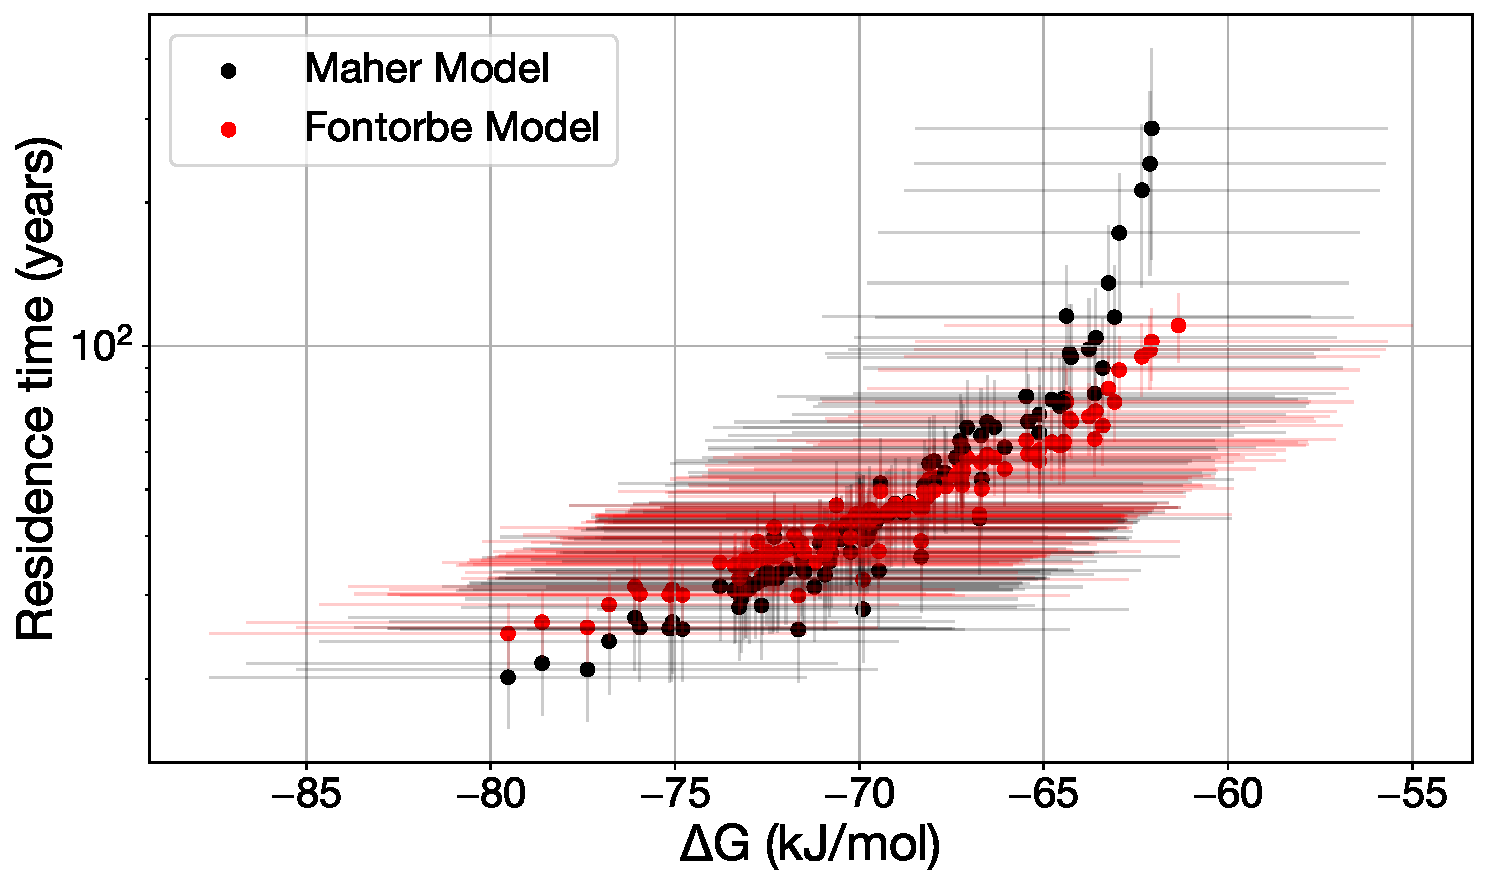
\includegraphics[width=0.9\textwidth]{delta_G_R_Si_time_Maher_vs_Fontorbe_Overlaid.pdf}
    \caption{Comparison of the delta G obtained against elevation. Comparison of delta G with residence time for both models}
    \label{fig:discussion11}
\end{figure}

\FloatBarrier

Calculated free energy shown in Figure \ref{fig:discussion11} shows that all springs in the catchment have a free energy that is more negative than -40 kJ/mol. These samples are therefore classified as far from equilibrium. Figure \ref{fig:discussion11} does show that free energy gets closer to zero as residence time increases. This is consistent with the notion that groundwaters approach equilibrium the more they stay in the subsurface and react. However, the extent of reaction is not great enough to be considered close to equilibrium. This suggests that, for Melamchi, using the Maher model to estimate residence times is not appropriate, and so the greatest control on weathering is temperature. This is more apparent when considering the residence times predicted at the sourthernmost Traverse 1.

\newpage

\subsection{Model Pitfalls}

Residence times in Traverse 1 are explainably the longest in the catchment. The springs here at are the lowest elevation, so the flow paths are presumably the longest. This is consistent with the highest DSi concentration of the catchment, and evidence for secondary precipitation of kaolinite at the lowest elevations (See Figure ?b). In Traverse 1, the Fontorbe model predicts a peak of $\approx$ 100 years, while the Maher model has a much higher residence time of $\approx$ 600 years. The discrepancy is likely due to how the models are formulated.

\begin{table}[h]
    \centering
    \renewcommand{\arraystretch}{2.2} % Adjust row spacing
    \begin{tabular}{cc}
        \toprule
        \textbf{Fontorbe} & \textbf{Maher} \\
        \midrule
        $\displaystyle T_f  = \frac{\left(C_h - C_o\right)\cdot\phi}{\left(1-f\right)\cdot R_n}$ & 
        $\displaystyle T_f = \frac{C_{eq} \cdot \left(C - C_0\right)}{e^2 R_n \left( C_{\text{eq}} - C \right)}$ \\ [10pt]
        \bottomrule
    \end{tabular}
    \caption{Comparison of equations from Fontorbe and Maher}
    \label{tab:equations}
\end{table}

The difference in the models comes from the underlying assumptions of reaction rate and how it changes towards equilibrium. Reaction rate is kept constant in the Fontorbe model assuming a far from equilibrium state. In the Maher model, reaction rate depends on the equilibrium concentration. It is unrealistic that reaction rate continue to be constant as the reaction progresses, and so the Maher model more accurately reflects water that is close to equilibrium. Indeed, as equilibrium concentration is reached in the Maher model, the reaction rate will decrease. In order to produce more concentrated springwaters as in Traverse 1, the groundwater must have a longer residence time. The $\frac{C_{eq}}{(C_{eq} - C)}$ term in the Maher model gets larger as the concentration approaches equilibrium. As a result of this, the Maher model consistently predicts longer residence times than the Fontorbe Model at higher DSi concentrations, while the opposite is true at lower DSi concentrations. It also follows that for Traverse 1 the $\frac{C_{eq}}{(C_{eq} - C)}$ term grows arbitrarily large, hence the strong discrepancy found in Figure (?c).

\bsk

For this study's calculations, the equilibrium concentration is taken to be the highest in the catchment, 869 $\mu$M DSi. This concentration corresponds the highest spring concentration found in Traverse 1. Note that in the Maher and Chamberlain (2014) model setup, an equilibrium concentration of 375$\mu$M DSi is chosen from the global river data of Gaillardet et al. (1999). This is sound for a theoretical model but is not appropriate for this catchment. It is unclear, however, whether choosing the highest DSi concentration in the catchment is appropriate. Clearly as this concentration is approached, the Maher model will predict unrealistic residence times, as shown in Figure \ref{fig:discussion11}. The free energy of the system suggests the spring system is far away from equilibrium, so choosing a larger $C_{eq}$ would produce better agreement with the Fontorbe model at higher DSi concentrations and allow for the calculated free energy. Additionally, Maher (2011) details several ways in which $C_{eq}$ could change depending on the conditions. For example, increasing PCO$_2$ would increase the concentration of DSi at equilibrium. However, if the Maher model assumes that all flow paths reach equilibrium, it is logical to use a concentration measured within the catchment; otherwise, applying the model would be of little relevance to the overall discussion on weathering controls.


\begin{figure}[h]
    \centering
    \includegraphics[width=0.8\textwidth]{TheoreticalCeq.pdf}
    \caption{Comparison of how concentration changes with flow path length for the two models, and different equilibrium concentration}
    \label{fig:discussion8}
\end{figure}

\FloatBarrier

There is another pitfall related to the dependence of residence time on the concentration of DSi. As is apparent in Figures ? ? ? ? and Equations ? ?, the estimated residence time of both models is directly related to the concentration of DSi in the spring water. This is by design, however as expressed in Subsection 6.1 (ref), low DSi is not necessarily indicative of less reacted groundwater. As a result of this, there is the possibility that the estimated residence times act more as a lower bound. A better approach in a future study could use elemental ratios, for example Na/Si that has a known behaviour as the reaction progresses. Elemental ratios would also factor out dilution as a potential influencing factor.



\newpage


\subsection{Significance of Free Energy for Reaction Rate}

Figure \ref{fig:discussion11} suggests that the system is far away from equilibrium, but the reaction rate constant used in both models for all calculations is one that is only considered feasible when close to equilibrium (Kampman et al., 2014). Both the Maher and Fontorbe model predict residence times consistent with the gas ages obtained by Atwood et al. (2021); it is just the free energy of reaction that allows for the conclusion that the greatest control on weathering in the catchment is temperature and not hydrology. In systems far from equilibrium, the reaction rate constant has been suggested to be much larger than those used in the models (Kampman et al., 2014). However, if the reaction rate is increased, the residence times predicted by the models will decrease. This is because the rate of reaction is inversely proportional to the residence time, as seen in the equations in Table \ref{tab:equations}. Reaction rate constants that are suggested to be far from equilibrium in Kampman et al. (2014) are laboratory-derived rates, and four orders of magnitude higher than those used in this study. Using these rates for the models predicts residence times in the range of 1-10 days. Under the assumption that the rates displayed Kampman et al. (2014) are accurate for systems far away from equilibrium, the results no longer agree with Atwood et al. (2021). Under these circumstances, then, the Maher and Fontorbe models are less likely to be appropriate for use in discussing weathering controls. 

\bsk

There are, however, counterarguments to this. Firstly, Kampman et al. (2014) investigates a catchment draining a different lithology, under different pH and pCO$_2$ conditions than Melamchi. Secondly, the reaction rate constants reported at far from equilibrium free energies are laboratory-calculated, at different conditions to both this study and Kampman et al. (2014). As discussed in the Introduction (ref), field derived reaction rate constants are often found to be lower than those measured in the lab. It is therefore unclear whether the k-$\Delta G$ relationship suggested in Kampman et al. (2014) is applicable to Melamchi, or natural catchments in general. In other words, in the absence of field-derived reaction rate constants in far from equilibrium settings, there is little evidence to suggest that the rate constants used in this study, and the models' calculated residence times are incorrect. This study therefore suggests that the Maher and Fontorbe models are appropriate for use in natural catchments like Melamchi, and that the greatest control on weathering is temperature.




\newpage

\section{Conclusions and Future Work}

Talk about using element ratios, and also isotope tracers eg Jotis, and also different reaction rates for forward and backward



% \bsk

% The consistency with which flow paths are sampled in Traverse 3 is more apparent when plotting Na/Si in one season against the rest (note that Figure \ref{fig:spatial_changes_spring8} the Na/Si values are uncorrected to showcase results collected in more than two seasons). 

% \begin{figure}[h]
%     \centering
%     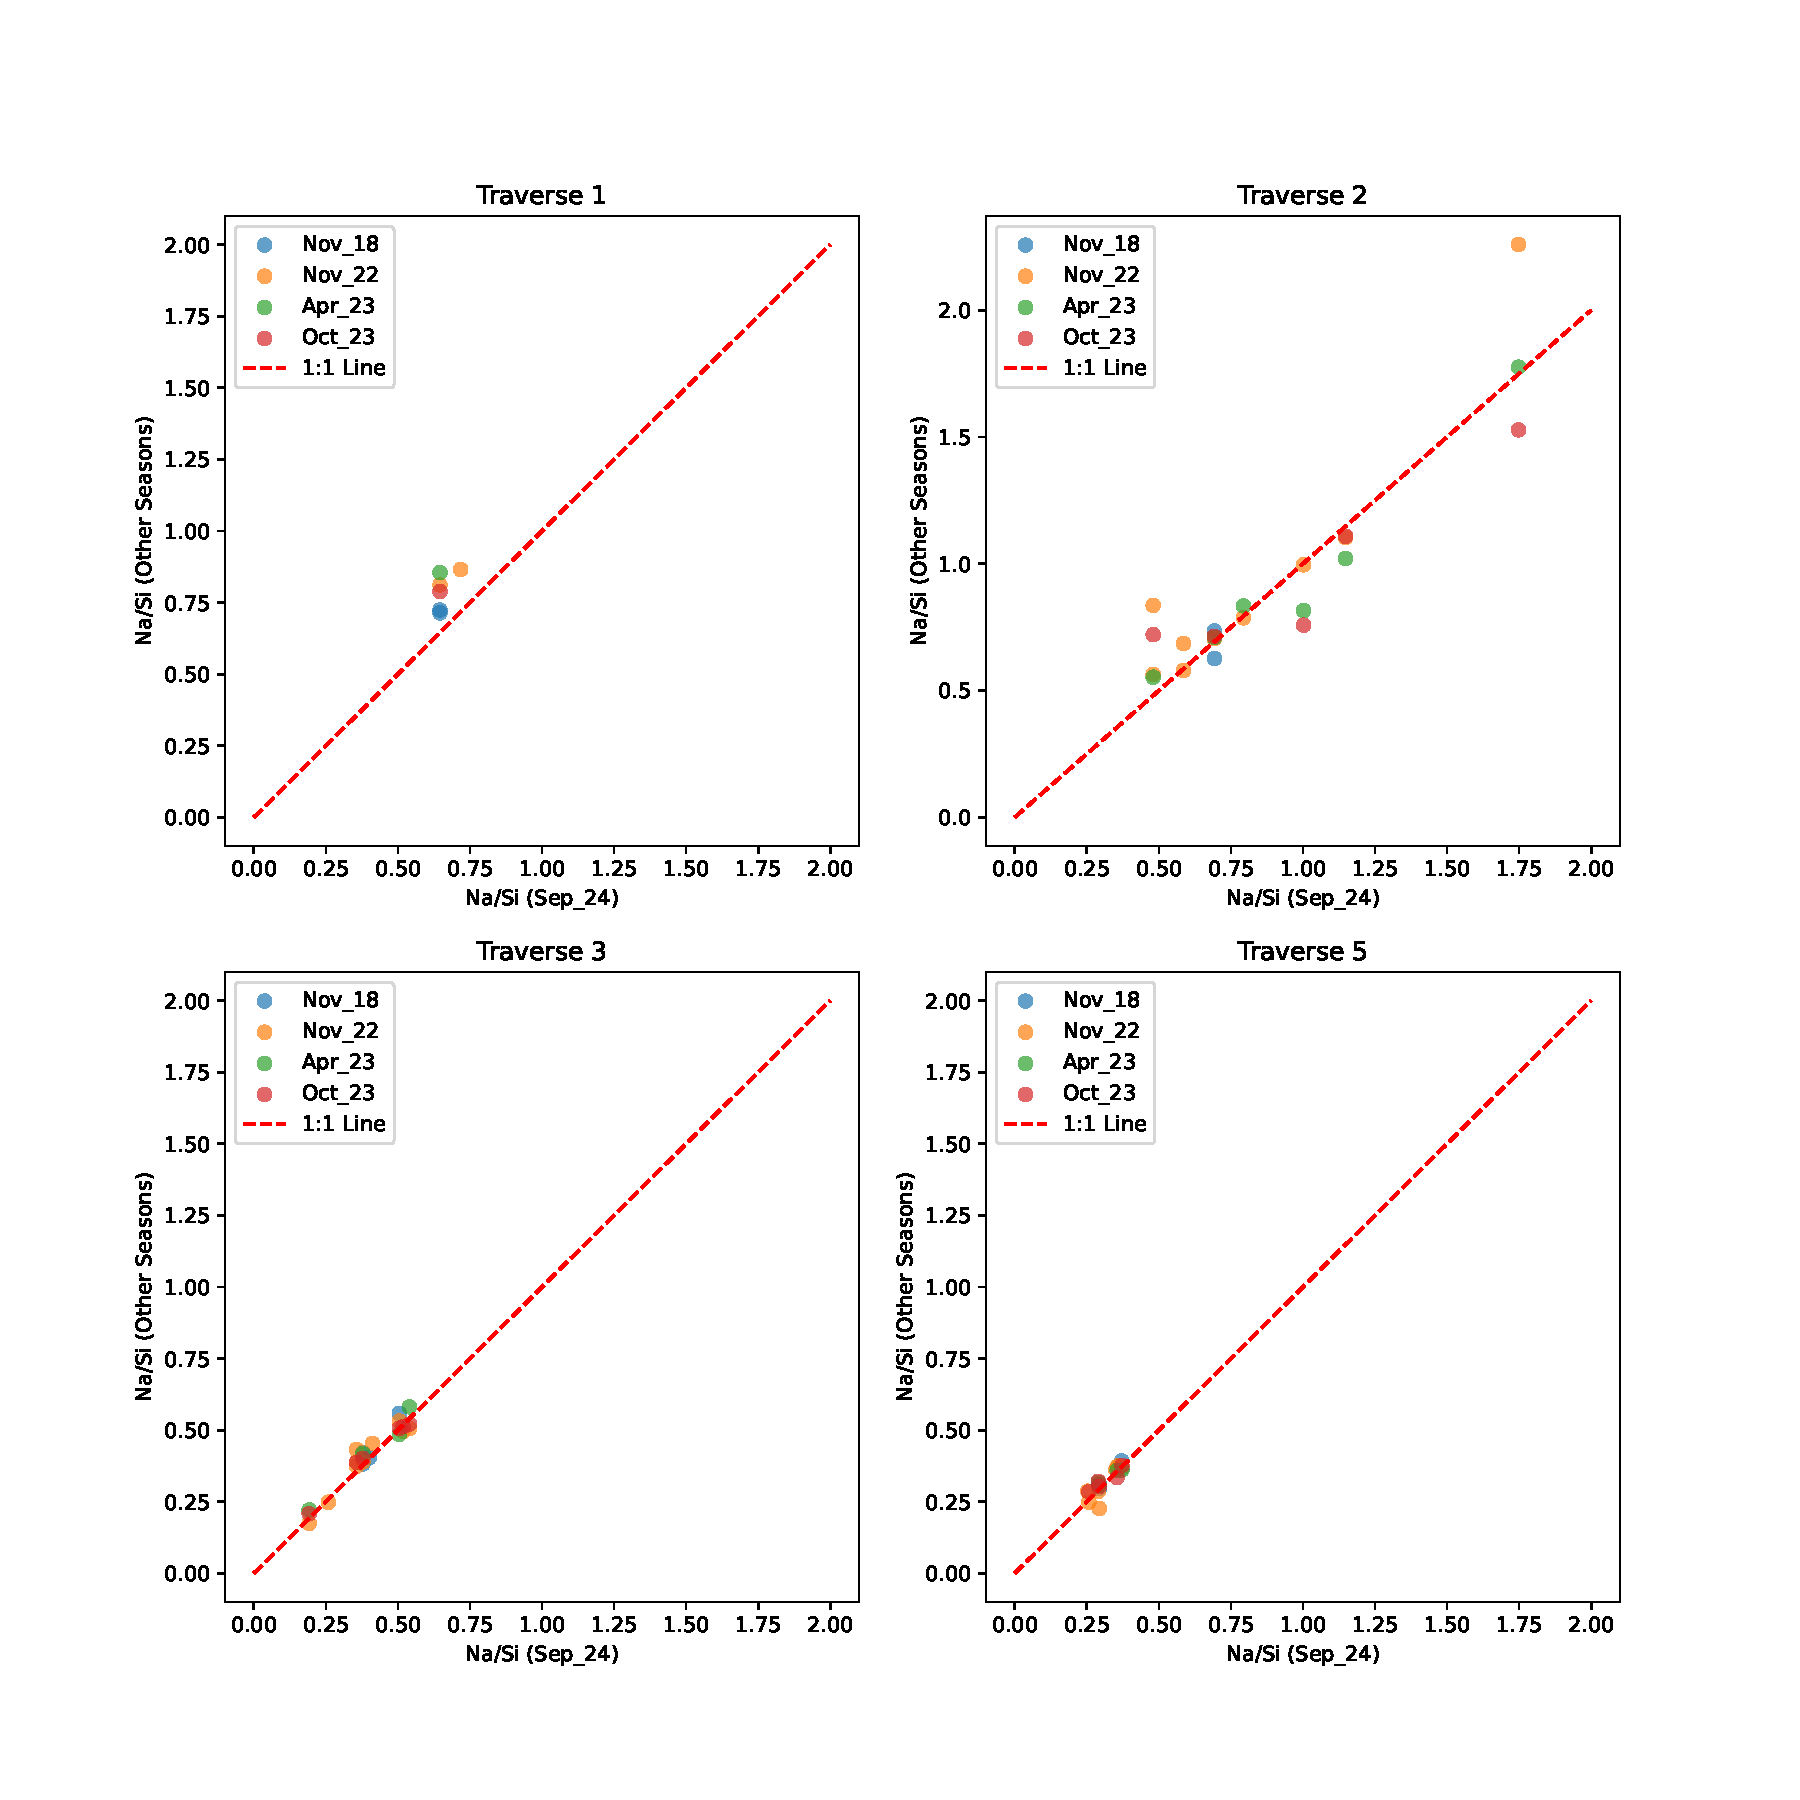
\includegraphics[width=\textwidth]{Na_Si_Seasons.pdf}
%     \caption{How Na/Si varies for different traverses. Traverse 4 is not plotted due to the lack of samples.}
%     \label{fig:spatial_changes_spring8}
% \end{figure}
% \FloatBarrier

% The scatter in these plots reflect temporal variability in the spring chemistry. Traverses 1 and 5 both display tight scatter, consistent with the notion that the flow paths here are consistently sampled. More notable here are the differences in Na/Si values between traverses. These how the spatial variability between traverses is more significant than the temporal variability. It is possible, and quite likely that all traverses flow paths are connected one to the other. When investigating model differences, however, a knowledge of which traverse accounts for what discrepancy allows for the contribution of spatial variation toward the overall interpretation to be taken into account.


% \subsection{Lithological Control on Spring Chemistry}

% Radiogenic strontium isotope analyses of springs show significant variation between different traverses. Sr isotope values of rain are consistent with the expected values for rainwater, with the exception of those sampled at low elevation (Galy, France-Lenord, Derry, 1999). The lowest Sr isotope value for rain is very close to the reported value for seawater, which is 0.70917 (Paytan et al, 2021). The rain samples with low strontium isotopic composition therefore indicate little contamination from dust or particles. Strontium isotope ratios used alongside strontium concentrations can be used to determine mixing between different endmembers (Faure, 1986; See Appendix). Plots of $\ddfrac{^{87}Sr}{^{86}Sr}$ against $\ddfrac{1}{Sr}$ that yield straight lines are indicative of mixing trends.


% \begin{figure}[p]
%     \centering
%     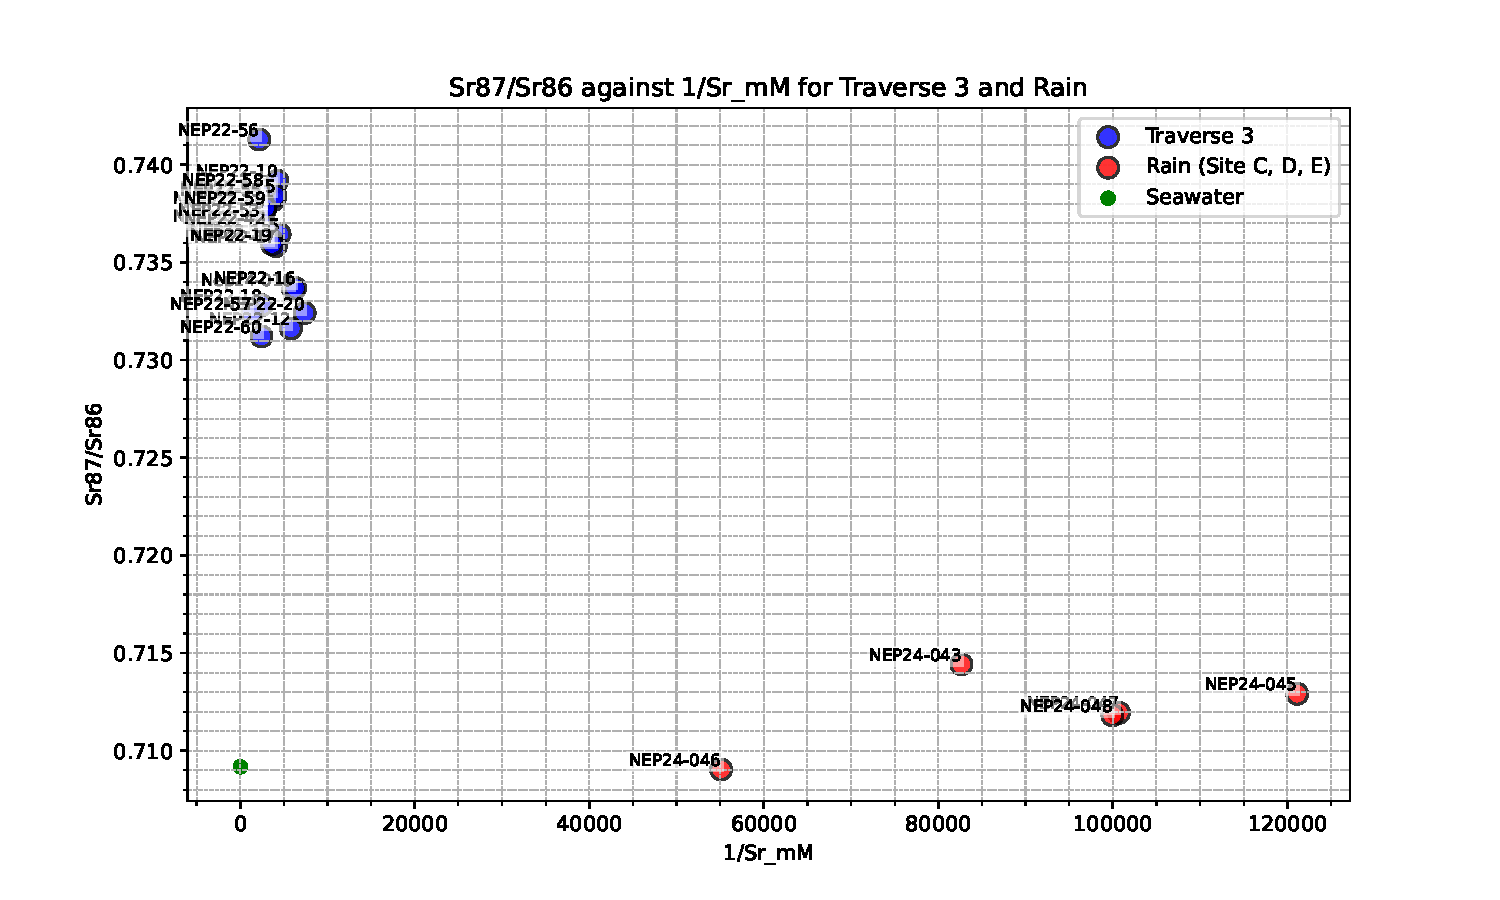
\includegraphics[width=\textwidth]{Sr87_Sr86_1Sr_Rain.pdf}
%     \caption{Strontium isotope differences display difference in lithology tapped in. Cite Quade and Tipper papers; Rain analysed for Sr isotopes and Cl. Something about contamination lower down; How samples of Traverse 3 compare to the rain samples}
%     \label{fig:discussion3}
% \end{figure}

% \FloatBarrier


% Comparing springs to rain in \ref{fig:discussion3}, the major control on spring chemistry does not appear to be the rain. Spring water mixing trends in $\ddfrac{^{87}Sr}{^{86}Sr}$ against $\ddfrac{1}{Sr}$ space are tightly scattered away from the rain. This suggests that rain input does not exert a significant control on the spring chemistry, which implies even the highest springs with the shortest flowpaths undergo significant weathering reactions with the rock. Instead, the water chemistry reflects that different traversal flowpaths sample lithologies that have different strontium isotopic composition. These variations are however within the range of Higher Himalayan Crystalline Series (HHCS) rocks found in the region, so this variation is to be expected (Tipper et al., 2006). It is unlikely that the source of the Sr isotopes is from the Lesser Himalayan Series (LHS) rocks, and the Main Central Thrust (MCT) is several km south of Melamchi.


